\subsubsection{Hidden Markov Model}
While Markov Models are very descriptive models of an environment, oftentimes when analyzing sound data, we do not have the information to paint the full picture. This means that we don\textquotesingle t have the full sequence of states, but we do have measurements from those states. Specifically, our states are the specific sounds that are made by an animal. We can call this a syllable (many bird songs consist of syllables). Unfortunately, we do not know these syllables, we only know the acoustic signals that they produce. These signals would be the evidence or observation in our current definition of the Hidden Markov Model (HMM). Using the sound waves we translated via Fourier transform, we can eventually get to the actual syllables made by the animal.\par

\begin{center}
  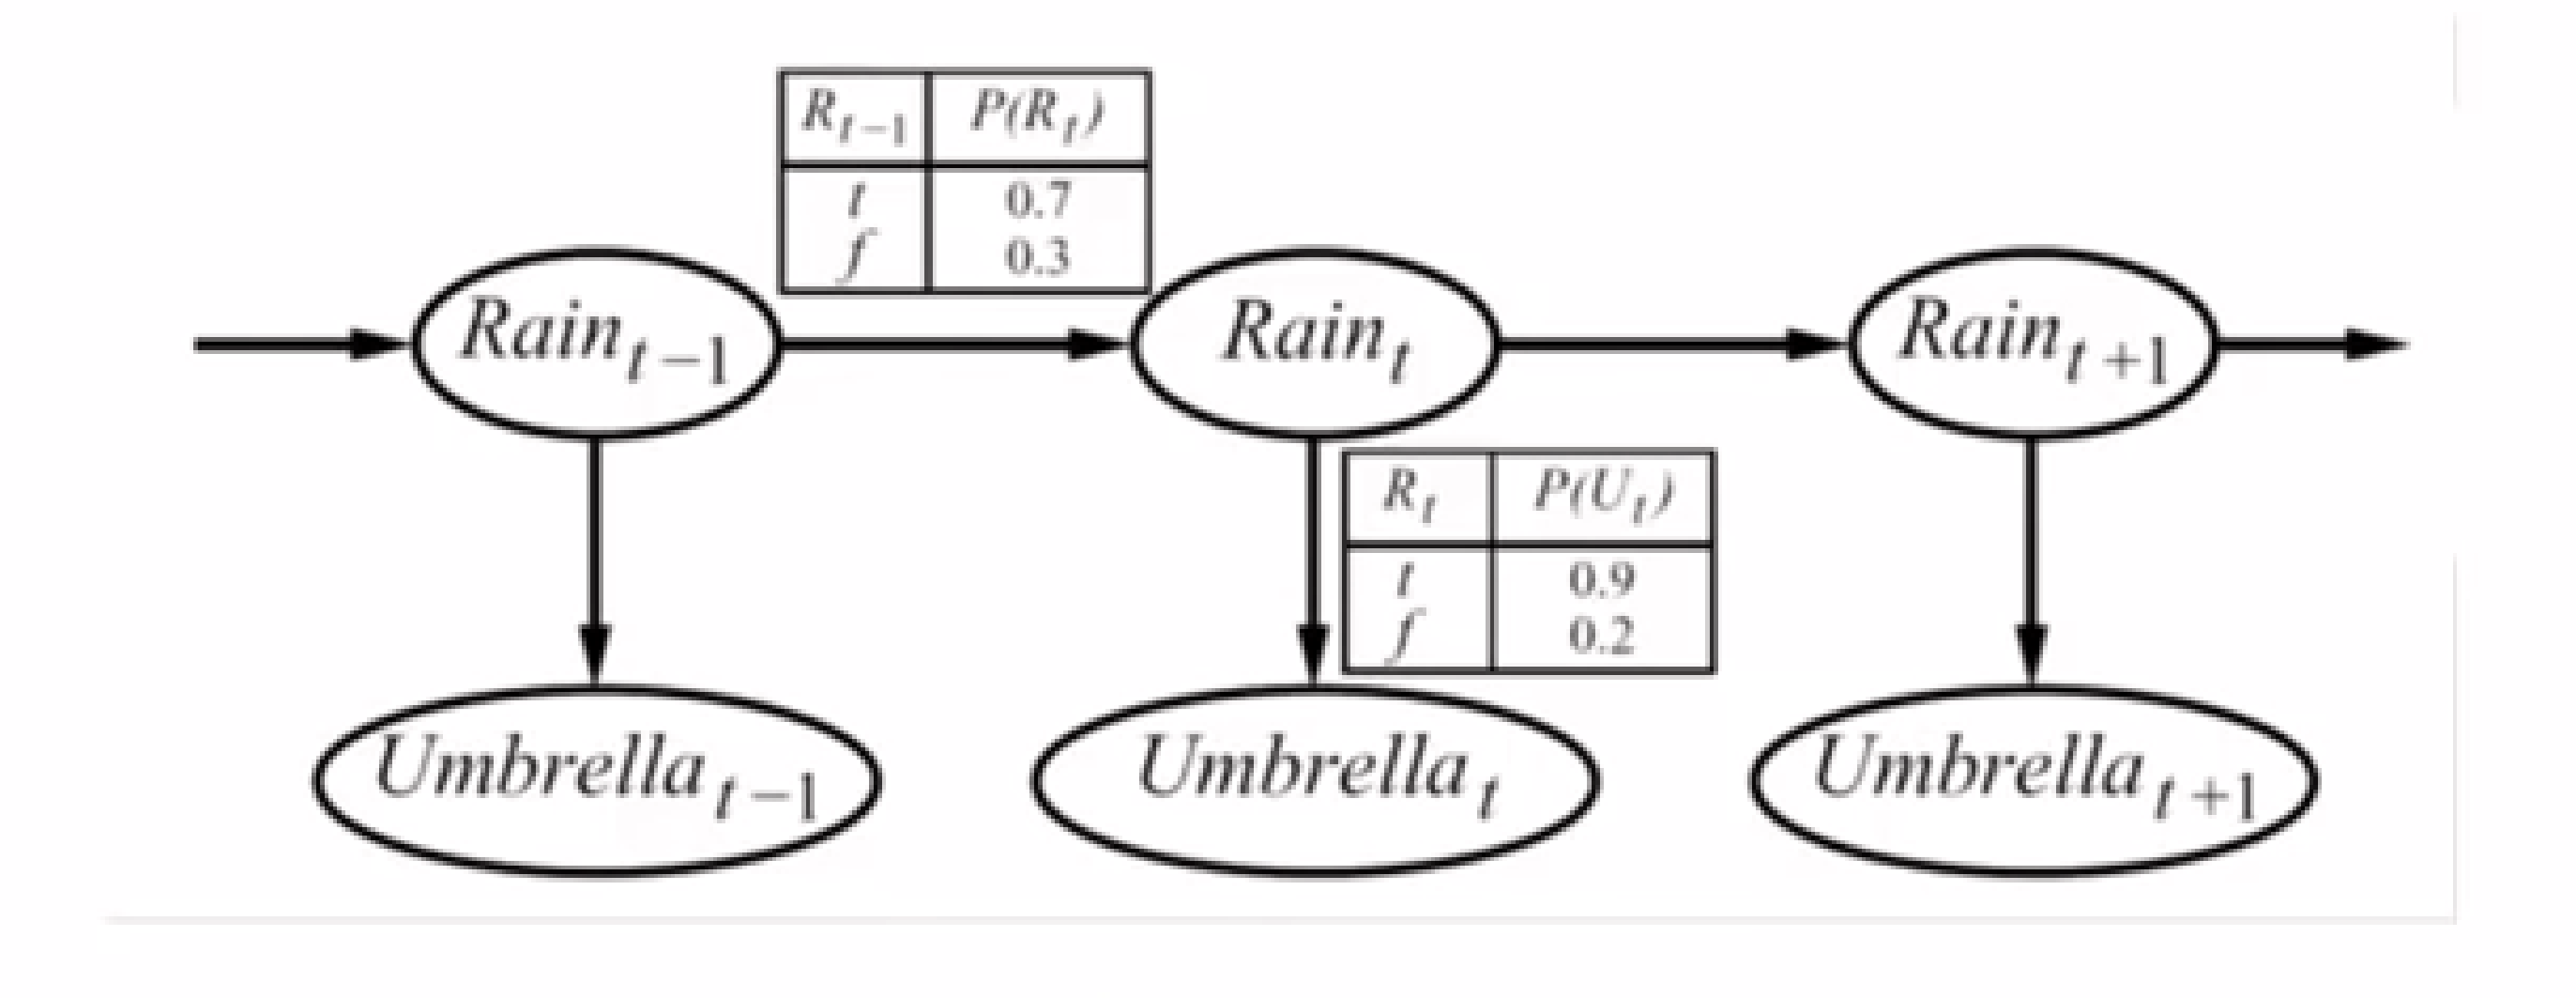
\includegraphics[width=\textwidth]{HMM}
\end{center}

When we talk about HMM, we are talking about the belief the current system is in. This is in reference to running an inference of the state based on what kind on evidence we have received. An example would be figuring that there is a 60\% chance that, with the current configuration of sound waves, syllable A is the sound made by the bird. This belief is obtained by filtering the current state with previous evidence. The method can be described by the following:\par

\begin{equation}
  B_{t}(X)
  = P_{t}(X_{t} | e_{1}, ..., e_{t})
  \textnormal{ where } e \textnormal{ is the evidence, }
  X \textnormal{ is the current state}
\end{equation}

We then update the belief via the following function:\par

\begin{equation}
  B'(X_{t+1})
  = P(X_{t+1} | e_{1}, ..., e_{t})
  = \sum_{X_{t}} P(X_{t+1} | X_{t}) P(X_{t} | e_{1}, ..., e_{t})
\end{equation}

We must then re-weight the likelihood of the current belief based on the probability of that belief state with the current evidence, using:

\begin{equation}
  B'(X_{t+1}) P(e_{t+1} | X_{t+1})
\end{equation}

The following image shows how HMM\textquotesingle s update their belief based off of time updates and then evidence updates.

\begin{center}
  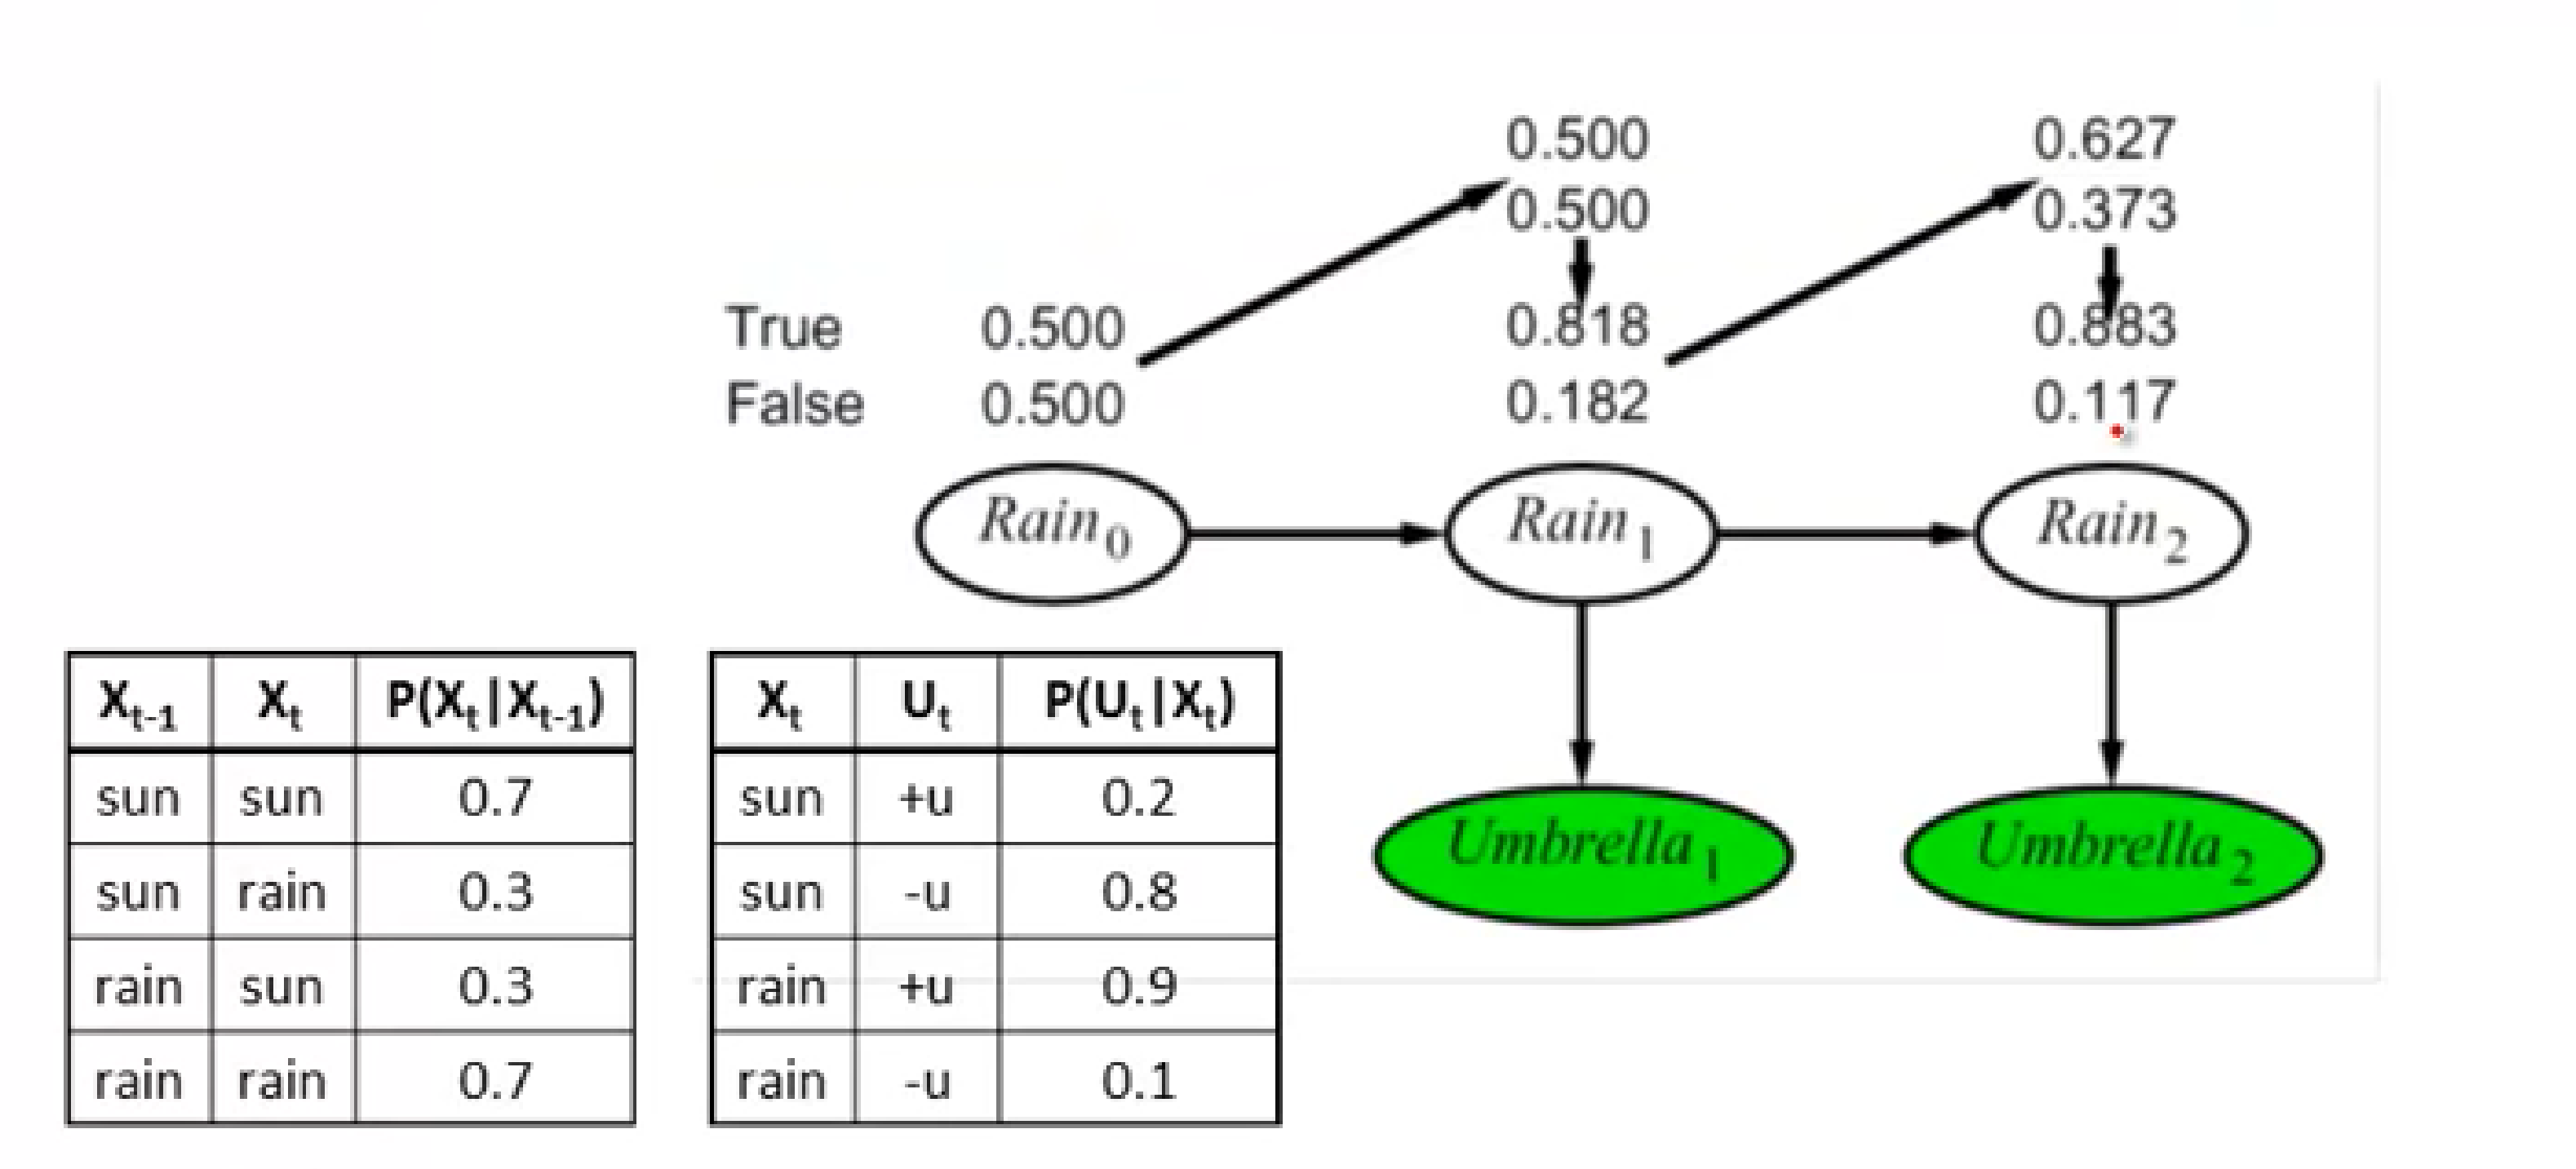
\includegraphics[width=\textwidth]{HMMupdate}
\end{center}
